
\section{Evaluation}
\label{sec:eval}
For the verification of the forecast, the model output data was evaluated against visibility measurements on the forecast domain. \\
In this section the measurement procedure for visibility is explained and the different scores used for the evaluation of the parametrizations are presented. \\ \\

\subsection{Measurements}
Visibility measurements are taken regularly at 6:00, 9:00, 12:00, 15:00 and 18:00 UTC, at each of the observation sites marked in Figure \ref{fig:stations}. The measurement is performed by a human observer, who identifies the most distant mark, which still can be seen \cite{WMO}. All horizontal directions need to be considered and the lowest value determines the visibility. The number-coded system for the categorization is presented in Table \ref{tab:synoptable} in Appendix \ref{sec:tabelappendix} and decreases in accuracy with increasing visibility. \\ 
The observational data is continuously stored in a joint database, where all national meteorological offices worldwide push their data.\\
Observations encoded by a different number-coded system, as found in Bosnia-Herzegovina and Serbia, were discarded. The data was further pre-selected by only using stations for the monthly average, which stably provided at least three measurements a day during the verification period. Additionally, it was tested if stations placed in a mountainous terrain showed a worse skill, because they were suspected of not being representative due to orographic mismatch, orographic shadowing or strong variations within a grid box. This turned out to have a negligible effect and as a result topological height was discarded as a selection criterion.

\begin{figure}[h]
    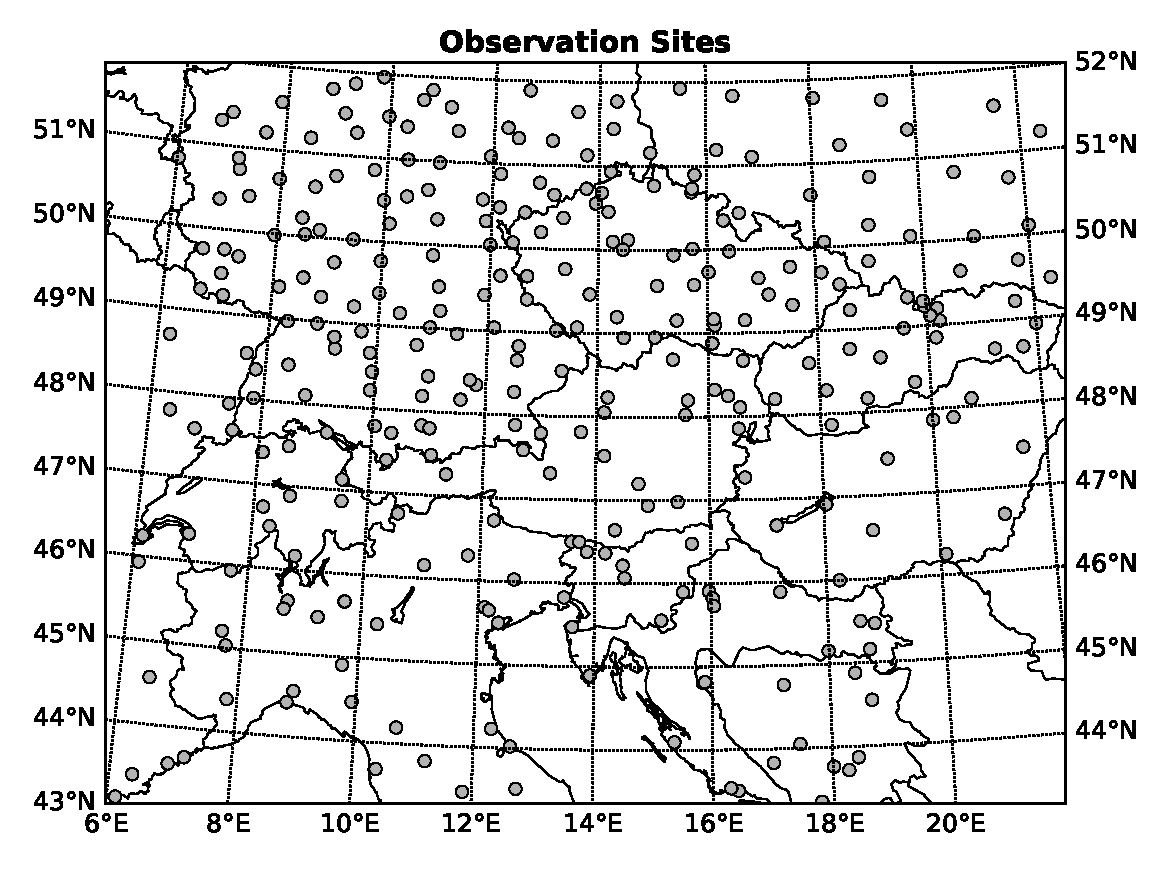
\includegraphics[width=\textwidth ] {graphics/Observation_Sites.eps}
    \caption[Map of Observation Sites]{Model domain and all observation sites where visibility measurements are taken}
    \label{fig:stations}
\end{figure}
 
\subsection{Scores}
For the computations of the scores only certain values on the model domain are used: The model output data for the forecast visibility is a two-dimensional field. For every station where visibility is measured, the data at the point of the coordinates of the measurement station was extracted from the two-dimensional field and evaluated. To obtain values for all coordinates of the stations, a nearest neighbour interpolation was performed. This was done for all points in time, when measurements are taken. Thus, the data can be index by time up to the number of all measurements within the verification period at one location $N_\mathrm{Mes}$ and by location up to the number of considered observations sites $N_\mathrm{S}$. \\
The different scores, we used for the evaluation of the goodness of the visibility prediction, are described in the following.\\

\subsubsection{Root Mean Squared Difference of the Logarithmic values (RMSLog) }
The average of the root-mean-square of the difference of the logarithm of the forecast and observed value is mathematically expressed as the following:
\begin{equation}
    \mathrm{RMSLog}_{n}(\lambda_{\mathrm{lon}}, \phi) =  \frac{1}{N_\mathrm{Mes}}\sum_{m=1}^{N_\mathrm{{Mes}}} \frac{ \sum_{i=1}^{N_{M_\mathrm{{tot}}}} (\log(vis_{\mathrm{o}_{n,m}}) - \log(vis_{\mathrm{f}_{i,n,m}}))^{2}} {N_{M_\mathrm{{tot}}}}
    \label{eq:haselstonerscore_loc}
\end{equation}

\begin{equation}
    \mathrm{RMSLog_{total}}=   \sqrt{\frac{ \sum_{n=1}^{N_\mathrm{S}} \mathrm{RMSLog}_{n} } {N_\mathrm{S}} } \quad .
    \label{eq:haselstonerscore_tot}
\end{equation}
To obtain a local score for each station $\mathrm{RMSLog}_{n}$, first, the average squared differences of the logarithmic values of the forecast visibility $vis_{\mathrm{f}_{i,n,m}}$ and the observed visibility $vis_{\mathrm{o}_{n,m}}$ are calculated. Here $i$ stands for the number of the member, $m$ indexes the time of the $m$th measurement and $n$ the location of the $n$th observation site.
First, the scores are averaged over the whole ensemble, where $N_{M_\mathrm{tot}}$ stands for the total number of ensemble members. Second, the average over all measurements in time is taken, where $N_\mathrm{Mes}$ stands for the number of measurements in the time span of interest.\\
To compute the total score $\mathrm{RMSLog_{total}}$, as described by Equation \eqref{eq:haselstonerscore_tot}, the root-mean-square of the mean of the local score $\mathrm{RMSLog}_{n}$ of the total number of stations $N_\mathrm{S}$ is taken.\\
The score, as described by Equation \eqref{eq:haselstonerscore_tot} and \eqref{eq:haselstonerscore_loc}, is computed from the logarithmic values with respect to the magnitude of the observed values: A forecast value that is off by 20km should be more weighted, when the observed value is 2km than, when it is 70km. Another reason for using a logarithmic score is that the observations are categorized with increasingly large intervals, so this way the different bin sizes of the measurement data (see Table \ref{tab:synoptable}) can be acknowledged.
\\

\subsubsection{Ranked Probability Score (RPS)}
The ranked probability score evaluates the probabilities gained from ensemble forecasting instead of only a mean value \cite{buizza1998impact}. Thus,  it is seen as a more accurate measure to test, if the perturbation scheme is well chosen. It is a commonly used score and described in the following after the textbook by \citeauthor{wilks2011statistical} \cite{wilks2011statistical}.\\
To calculate the RPS, first, the forecast values need to categorized into $K$ different bins. The number of ensemble members $N_{\mathrm{bin}_{j},M}$, whose predicted values are categorized in one bin, needs to be counted for a number of specified points in space and time for all bins. The points are chosen with respect to the available measurements, usually overlapping with their location and timing. As described by Equation \eqref{eq:card_mem}, the condition for a member being included in the count, the forecast values $f$ (in our case $vis_{\mathrm{f}_{i,n,m}}$ ) $\mathrm{bin}_{j,\mathrm{min}} < f < \mathrm{bin}_{j,\mathrm{max}}$ needs to be satisfied.
\begin{equation}
    N_{\mathrm{bin}_{j},M}(\lambda_{\mathrm{lon}}, \phi, t) = | \ \mathrm{mem} : f (\lambda_{\mathrm{lon}}, \phi, t) \in [\mathrm{bin}_{j,\mathrm{min}}, \mathrm{bin}_{j,\mathrm{max}}] \ |
    \label{eq:card_mem}
\end{equation}
From that, the forecast probability of an observation that lies within the interval of the $j$th bin is calculated as
\begin{equation}
 p_{\mathrm{bin}_{j}}(\lambda_{\mathrm{lon}}, \phi, t) = \frac{ N_{\mathrm{bin}_{j},\mathrm{M}} (\lambda_{\mathrm{lon}}, \phi, t)}{ N_{\mathrm{M_{tot}}}} \quad .
\end{equation}
For the RPS, the accumulated probabilities
\begin{equation}
 F_{J}=\sum_{j=1}^{J}  p_{\mathrm{bin}_{j}}
\end{equation}
and accumulated observations
\begin{equation}
 O_{J}=\sum_{j=1}^{J}  o_{\mathrm{bin}_{j}}
\end{equation}
 are used, where $o_{j}$ stands for the occurrence of an event. So if the observed value lies in the interval of the $j$th bin it equals 1, otherwise 0. A consequence of calculating a score from the accumulated probabilities is, that the higher the bin index $j$ is, the less is the accuracy of the bin weighted in the score. Like for the RMSLog, this is a desired property, because the accuracy of the visibility forecasts is more important for low values. Finally, we can define the RPS as
\begin{equation}
    \mathrm{RPS}=\sum_{J=1}^{K} \left( F_{J} - O_{J} \right)^{2} \quad .
    \label{eq:RPS}
\end{equation}
The conditions $ \sum_{j=1}^{K}  p_{\mathrm{bin}_{j}}=1 $ and  $ \sum_{j=1}^{K}  o_{\mathrm{bin}_{j}}=1 $ must hold and consequently, the last term of Equation \eqref{eq:RPS} always vanishes \parencite{wilks2011statistical}.\\
The bin edges for the RPS were defined as: [0.0, 0.5, 1.0, 5.0, 10.0, 15.0, 20.0, 30.0, 50.0, 80.0 ]. The increasing bin size relates to the decrease in accuracy in the number-coded system for the measurement data (Table \ref{tab:synoptable} in Appendix \ref{sec:tabelappendix}).
RMSLog and RPS show a high sensitivity to distance.\\ \\


A major concern when evaluating new parametrizations is, to not assess the performance of the whole model, but only of the parametrization. \\
This problem arises, because for certain days and weathers situations, the forecasts as a whole are bad, and since the visibility forecast uses other model variables as input, the total scores in visibility reflect also the overall model performance. 
The unbiased evaluation of parametrizations can never be achieved to perfection, but a thorough preselection of data can help. For this, the scores can be computed using only data of dates, where the overall model skill was high, or  the correlations of the skill of different model variables and the forecast variable we want to assess can be analysed.\\
Another way to tackle this problem is, to use a relative score. Meaning, if a comparable parametrization already exists, the quality of the forecasts is only quantified in terms of relative improvement.
The Gul-parametrization was so far the only tool for visibility prediction and already implemented in a post-processing package for AROME at ZAMG. Therefore, we decided to evaluate the other parametrizations against the Gul-parametrization (see Table \ref{tab:Paraoverview}).\\
In order to do so, a relative version of the RMSLog and the RPS are introduced. 
For the RMSLog and the RMSE, the relative score is expressed in percentage of the total score of the Gul-parametrization.
For the RPS, the relative version is given by the Ranked Probability Skill Score (RPSS). The RPSS is a traditional skill score. A skill score SS is generally defined as 
\begin{equation}
    \mathrm{SS}=\frac{\mathrm{A}- \mathrm{A_{ref}}}{\mathrm{A_{perf}} - \mathrm{A_{ref}}}
\end{equation}
(e.g. \citeauthor{wilks2011statistical} \cite{wilks2011statistical} ), where A stands for the accuracy. $\mathrm{A_{ref}}$ is the accuracy of the reference case  and $\mathrm{A_{perf}}$ the accuracy of a perfect forecast.
That means that the goodness of the parametrization is rated with respect to a reference parametrization that has a ranked probability score $\mathrm{RPS_{ref}}$. The RPS of the other parametrization is evaluated against it, as described by 
\begin{equation}
    \mathrm{RPSS} = 1 - \frac{\mathrm{RPS}}{\mathrm{RPS}_\mathrm{ref}} \quad ,
    \label{eq:RPS_skill}
\end{equation}
since for the RPS  the perfect accuracy $\mathrm{A_{perf}}$ equals 0. Regarding Equation \eqref{eq:RPS_skill} it is evident that the RPSS has to lie within the interval $[- \infty, \ 1]$ and all values greater than zero indicate a better performance, than the one of the reference. 